% Created 2021-02-28 Sun 22:59
% Intended LaTeX compiler: pdflatex
\documentclass[11pt]{article}
\usepackage[utf8]{inputenc}
\usepackage[T1]{fontenc}
\usepackage{graphicx}
\usepackage{grffile}
\usepackage{longtable}
\usepackage{wrapfig}
\usepackage{rotating}
\usepackage[normalem]{ulem}
\usepackage{amsmath}
\usepackage{textcomp}
\usepackage{amssymb}
\usepackage{capt-of}
\usepackage{hyperref}
\date{\today}
\title{}
\hypersetup{
 pdfauthor={},
 pdftitle={},
 pdfkeywords={},
 pdfsubject={},
 pdfcreator={Emacs 27.1 (Org mode 9.4.4)}, 
 pdflang={English}}
\begin{document}

\tableofcontents

\newpage
\section{System Requirements}
\label{sec:org743dbd9}
\begin{itemize}
\item Works on all major operating systems
\item Java version 11-15
\end{itemize}
\section{How to Use TAB2XML}
\label{sec:org87d8fb1}
\subsection{Installation}
\label{sec:orge1b5e53}
\subsubsection{Eclipse}
\label{sec:org06e14fd}
\begin{enumerate}
\item Open Eclipse, and press \texttt{File > Import} in the menus.
\begin{center}
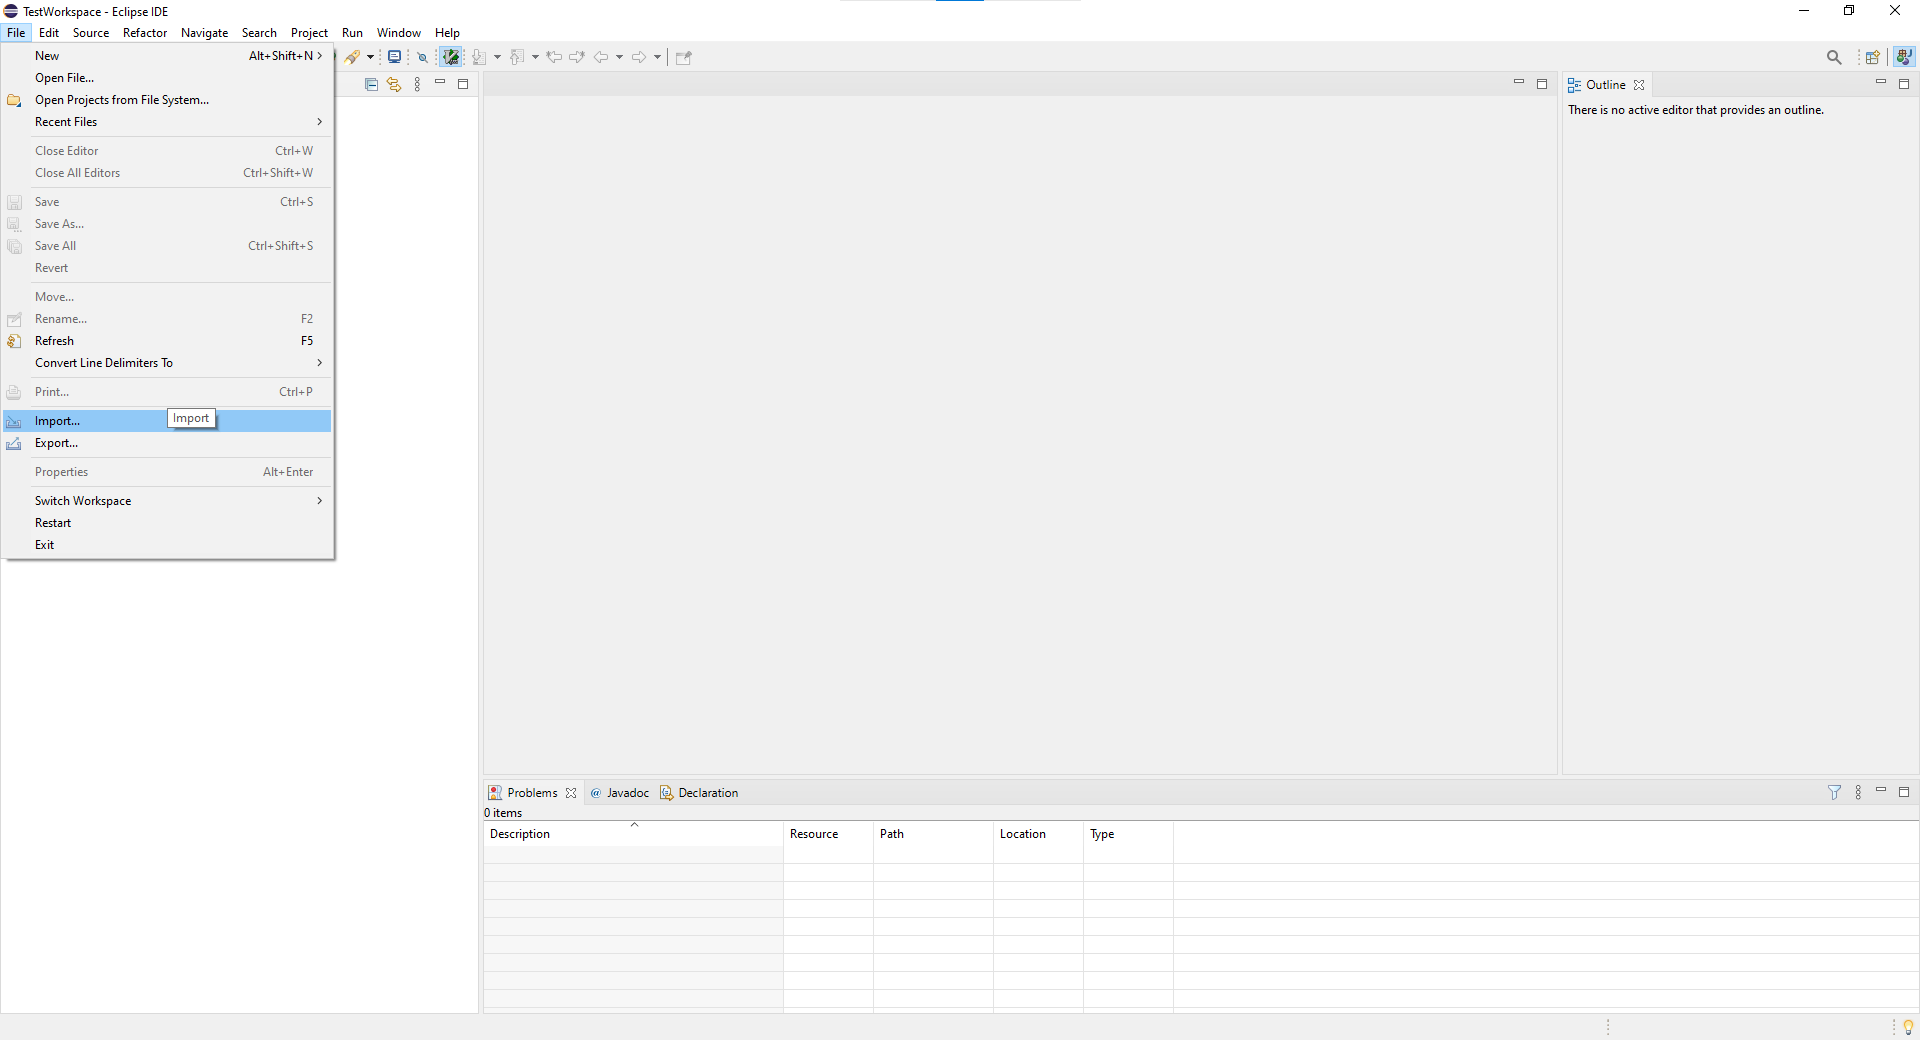
\includegraphics[width=.9\linewidth]{../Screenshots/eclipse-install-1.png}
\end{center}
\item In the window that opens, select "Projects from Git", in the folder called "Git".  Then, click "Next"
\begin{center}
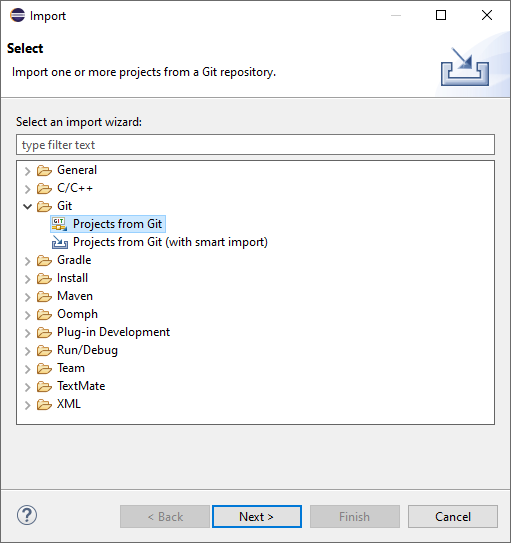
\includegraphics[width=.9\linewidth]{../Screenshots/eclipse-install-2.png}
\end{center}
\item Click "Clone URI" then click "Next".
\begin{center}
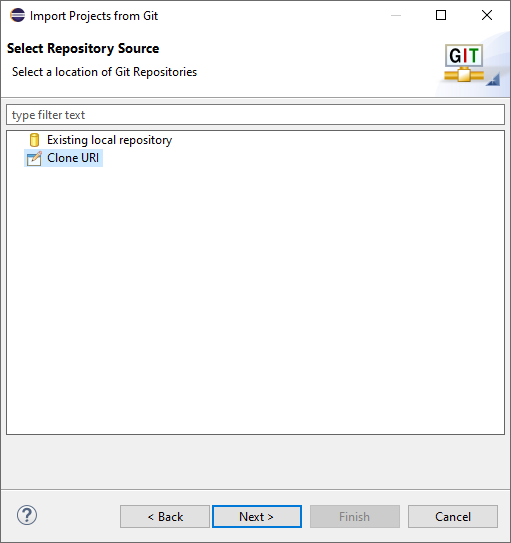
\includegraphics[width=.9\linewidth]{../Screenshots/eclipse-install-3.png}
\end{center}
\item Enter "\texttt{https://github.com/ahopk127/eecs2311-tab2xml.git}" in the first field ("URI"), then click "Next".  No authentication is required.
\begin{center}
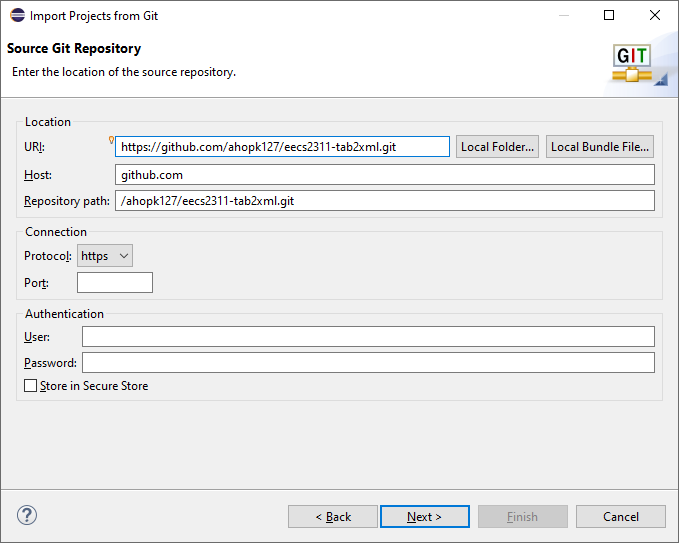
\includegraphics[width=.9\linewidth]{../Screenshots/eclipse-install-4.png}
\end{center}
\item Choose where you want the program to be saved on your computer (or just use the default location), then click "Next".
\begin{center}
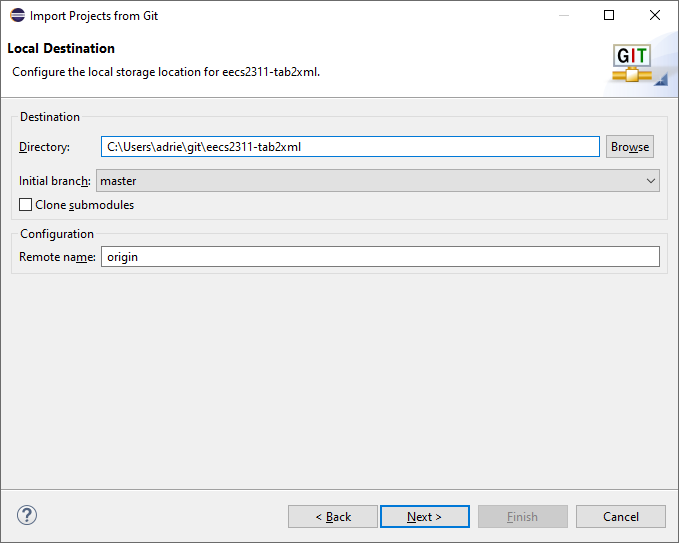
\includegraphics[width=.9\linewidth]{../Screenshots/eclipse-install-5.png}
\end{center}
\item Click "Next" then "Finish".  The program is now installed on your computer, but must be built using Gradle.
\begin{center}
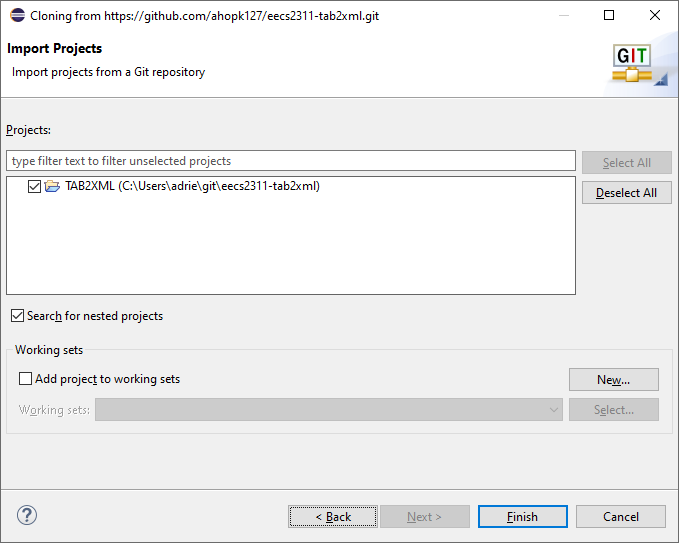
\includegraphics[width=.9\linewidth]{../Screenshots/eclipse-install-7.png}
\end{center}
\item You will need the "Gradle Tasks" window for the next step.  If you can't find it, press \texttt{Window > Show View > Other} in the menu, then find "Gradle Tasks" in the Gradle folder, then click "Open".
\begin{center}
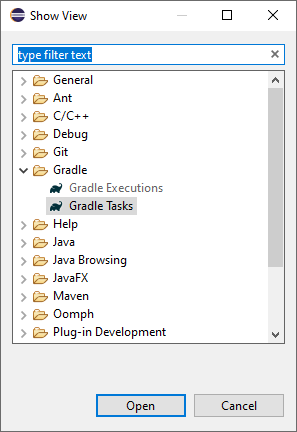
\includegraphics[width=.9\linewidth]{../Screenshots/eclipse-build-2.png}
\end{center}
\item In the "Gradle Tasks" window, double-click the green "build" item in the "build" folder.
\begin{center}
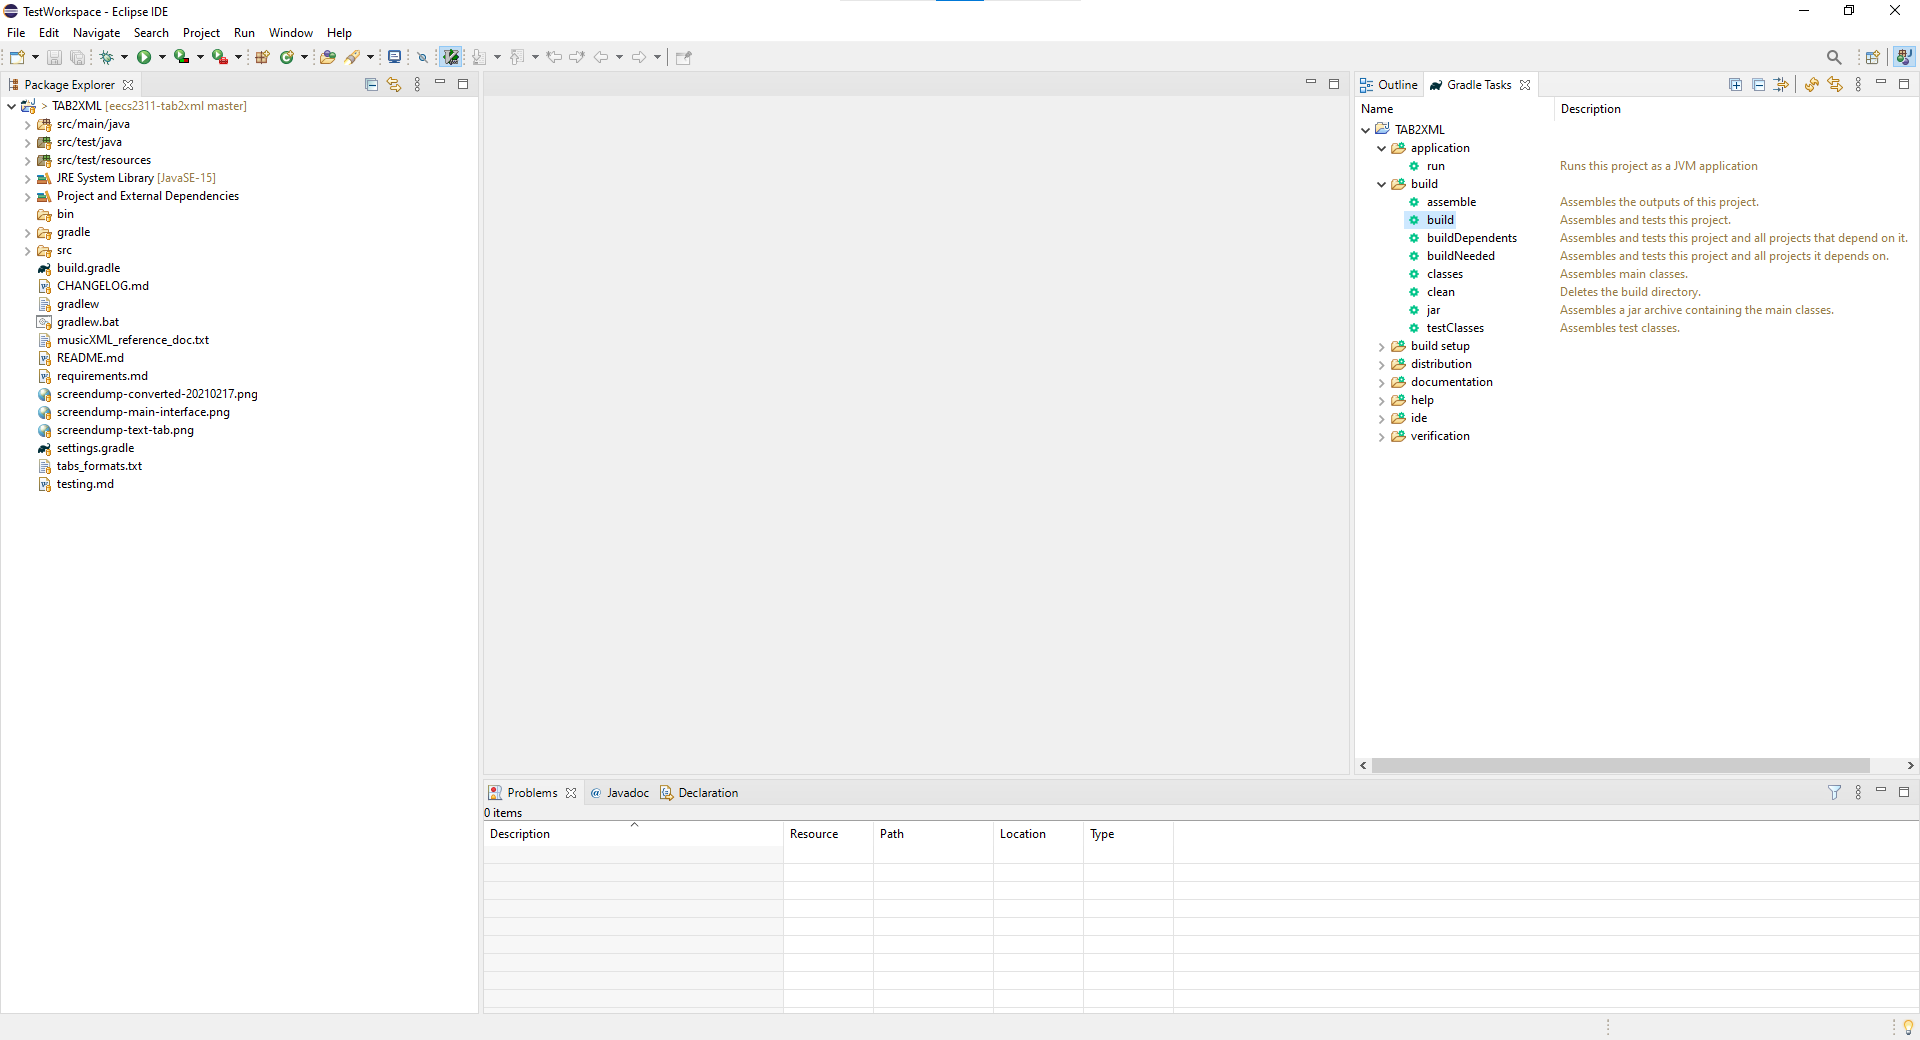
\includegraphics[width=.9\linewidth]{../Screenshots/eclipse-build.png}
\end{center}
\end{enumerate}
\subsubsection{Commandline}
\label{sec:orgce43265}
\begin{enumerate}
\item Use the command \texttt{git clone https://github.com/ahopk127/eecs2311-tab2xml.git} to clone the project to the directory of your choice
\item Change directory to the directory where you installed the project, then use \texttt{./gradlew build} to build the project.
\end{enumerate}
\subsection{Convert Text Tab}
\label{sec:org7bda3dc}
\begin{enumerate}
\item Run the application.  In Eclipse, double-click the green "run" item in the "application folder".  In commandline, use \texttt{gradlew run}.\\
You should see a window like this:
\begin{center}
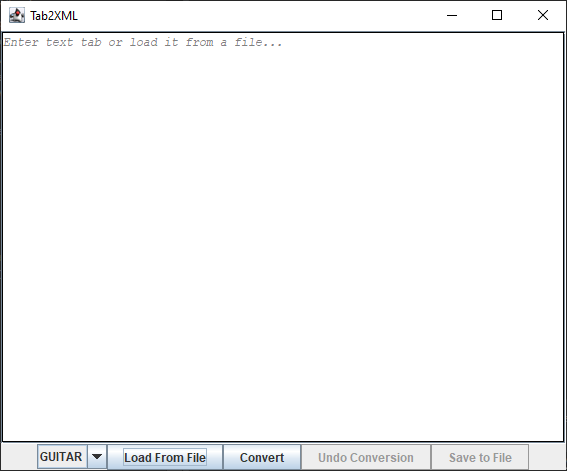
\includegraphics[width=.9\linewidth]{../Screenshots/main-interface.png}
\end{center}
\item Input your text tab into the application.  There are multiple ways of doing this:
\begin{itemize}
\item Type or copy-and-paste your text tab into the text box.
\item Press the "Load from File" button then choose a file to load your text tab from a file.
\item Drag and drop a text tab file into the input box
\end{itemize}
\begin{center}
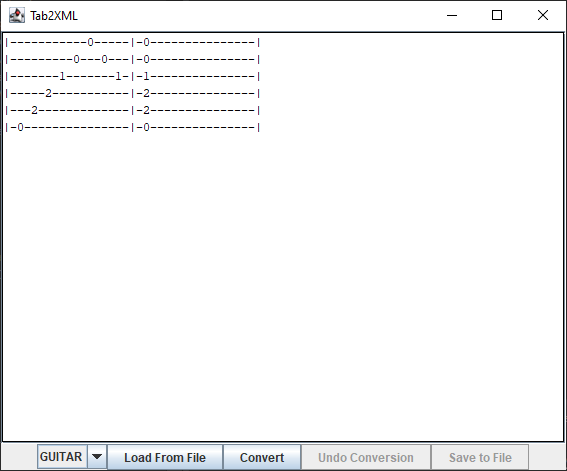
\includegraphics[width=.9\linewidth]{../Screenshots/text-tab.png}
\end{center}
\item Press the "Convert" button.  The text tab will be replaced with the corresponding MusicXML.
\begin{center}
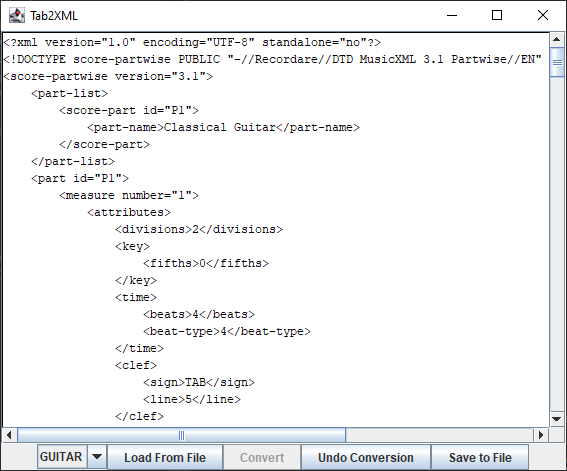
\includegraphics[width=.9\linewidth]{../Screenshots/converted-20210217.png}
\end{center}
\item You can now copy-and-paste the MusicXML, or save it to a file using the "Save to File" button.
\end{enumerate}
\subsection{Other Use Cases}
\label{sec:orge94bb2c}
\begin{itemize}
\item You can use the "Convert and Save" button to convert a text tab and save it to a file in one step.  In addition, the tab in the input box will not be replaced with MusicXML, so you can edit it then convert again!
\item After converting text tab with the "Convert" button, you can press the "Undo Conversion" button to go back to the original text tab.
\item To clear the text box, press Ctrl-A then Delete.  If you want to load in another text tab, you don't need to do this.  Simply press "Load from File" to load another text tab.
\end{itemize}
\subsection{How to Use in Code}
\label{sec:org81632bc}
If you would like to use this project in your own program, the following code can be used to convert tab to MusicXML:

\begin{verbatim}
tab2xml.parser.Parser parser = new tab2xml.parser.Parser(INPUT, INSTRUMENT);  
String output = parser.parse();  
\end{verbatim}

Notes:
\begin{itemize}
\item INPUT is the text tab.  It should be a \texttt{String}, not a file.
\item INSTRUMENT is the instrument the tab is for.  It should be an instance of \texttt{tab2xml.parser.Instrument}.
\item You will need to handle the checked exceptions thrown by \texttt{Parser.parse()}
\end{itemize}
\end{document}
